\chapter{Literature review}
    
    Before moving into the different cases and simulations carried out, an extensive analysis of the current state-of-art must be done: begging from the basics and going through the latest papers. The study will be structured in the three main parts of the thesis: optimization of multi-objective problems, genetic algorithms and computer fluid dynamics.

\section{Optimization}

    Most parts of the real-life engineering problems face not one but more variables to be optimized. The value of those variables is tried to be minimized or maximized depending on the case. However, in both cases, the idea is to get the optimum value. Those kind of problems are called \textit{multi-objective optimization} given that there is more than one objective that is wanted to be optimized. The main difficulty is that those objectives are usually in conflict with each other, i.e. there is not a point where the solution is optimal (in the sense that it minimizes/maximizes all the objectives).
    
    The formal definition of multi-objective optimization is \cite{nonlinear}:
    \begin{equation}
        \begin{array}{cl}
            \textrm{minimize} & \{f_1(\bm{x}),f_2(\bm{x}),...,f_k(\bm{x})\} \\
            \textrm{subject to} & \bm{x} \in S
        \end{array}
        \label{eq:multiobjectiveDefnition}
    \end{equation}
    where there are $k$ objective functions that should be minimized ($k > 2$). The decision vector $\bm{x}$ contains the $n$ variables $\bm{x}=(x_1,x_2,...,x_n)$ of the $k$ functions and it must belong to a nonempty set $S$ of the search space. $S$ is also called the feasible set of the search space and it is usually described by constraint functions (in addition to some upper and lower bounds for each variable). Optimization problems are usually described to minimize a function, but maximize the function $f_i(\bm{x})$ is equivalent to minimize the function $-f_i(\bm{x})$.
    
    \newpage
    
    It must be noted that there are two spaces in which the optimization works: parameter or search space (denoted with $S$ in the literature) and optimization, objective or function space (denoted with $Z$). These different designations will be interchangeable during the oncoming discussion. 
    
    \begin{figure}[h!]
        \centering
        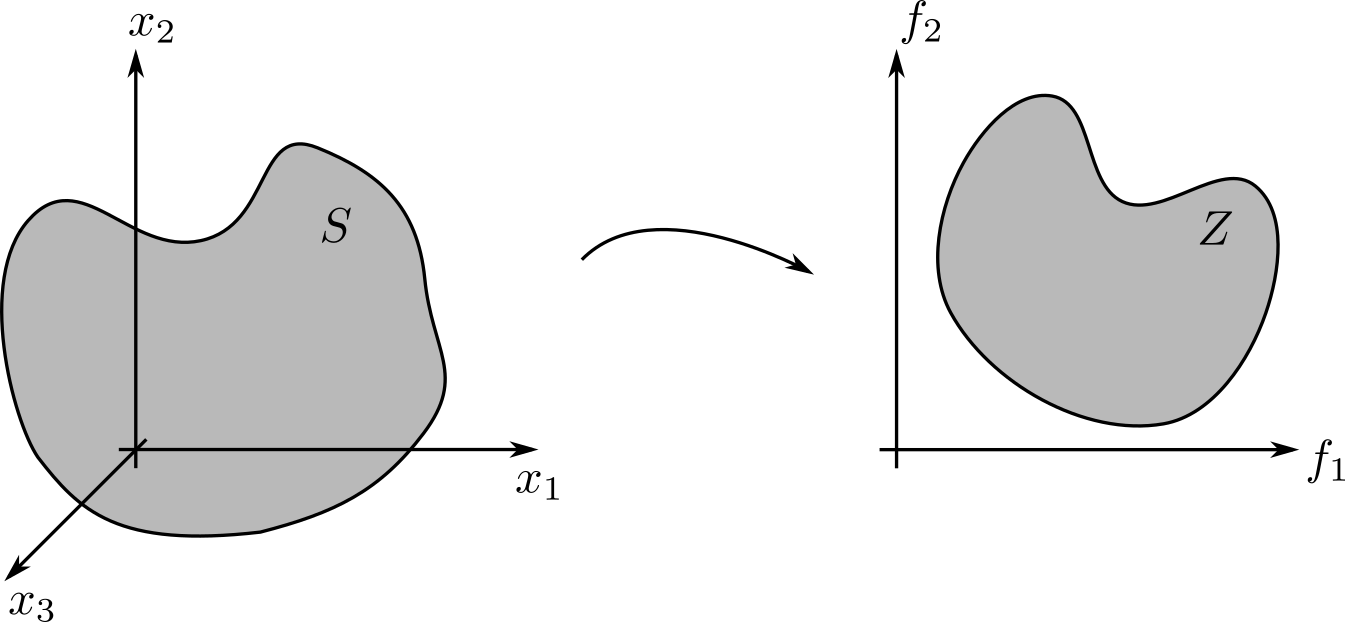
\includegraphics[width=0.8\textwidth]{Figures/2/searchSpaceFunction.png}
        \caption{Search ($S$) and function ($Z$) space in multi-objective optimization}
        \label{fig:twoSpaces}
    \end{figure}    
    
    A visual example of this kind of problems can be seen in figure \ref{fig:BihnKorn}, where the test function proposed by Binh and Korn (Test Case 2 from \cite{binh1997mobes}) is plotted. The function was stated as:
    \begin{equation}
        \begin{array}{cl}
            \textrm{minimize} & 
            \left\{ \begin{array}{l}
                f_1(x_1,x_2) = 4x_1^2 + 4x_2^2\\
                f_2(x_1,x_2) = (x_1-5)^2+(x_2-5)^2
            \end{array} \right. \\
            & \\
            \textrm{subject to} &  
            \left\{ \begin{array}{l}
                (x_1-5)^2+x_2^2-25 \leq 0\\
                -(x_1-8)^2-(x_2+3)^2 + 7.7 \leq 0
            \end{array} \right. \\
            & \\
            \textrm{bounded by} & -15 \leq x_i \leq 30, \ \ \forall i = 1,2
        \end{array}
        \label{eq:BihnKorn}
    \end{equation}
    
    \begin{figure}[h!]
        \centering
        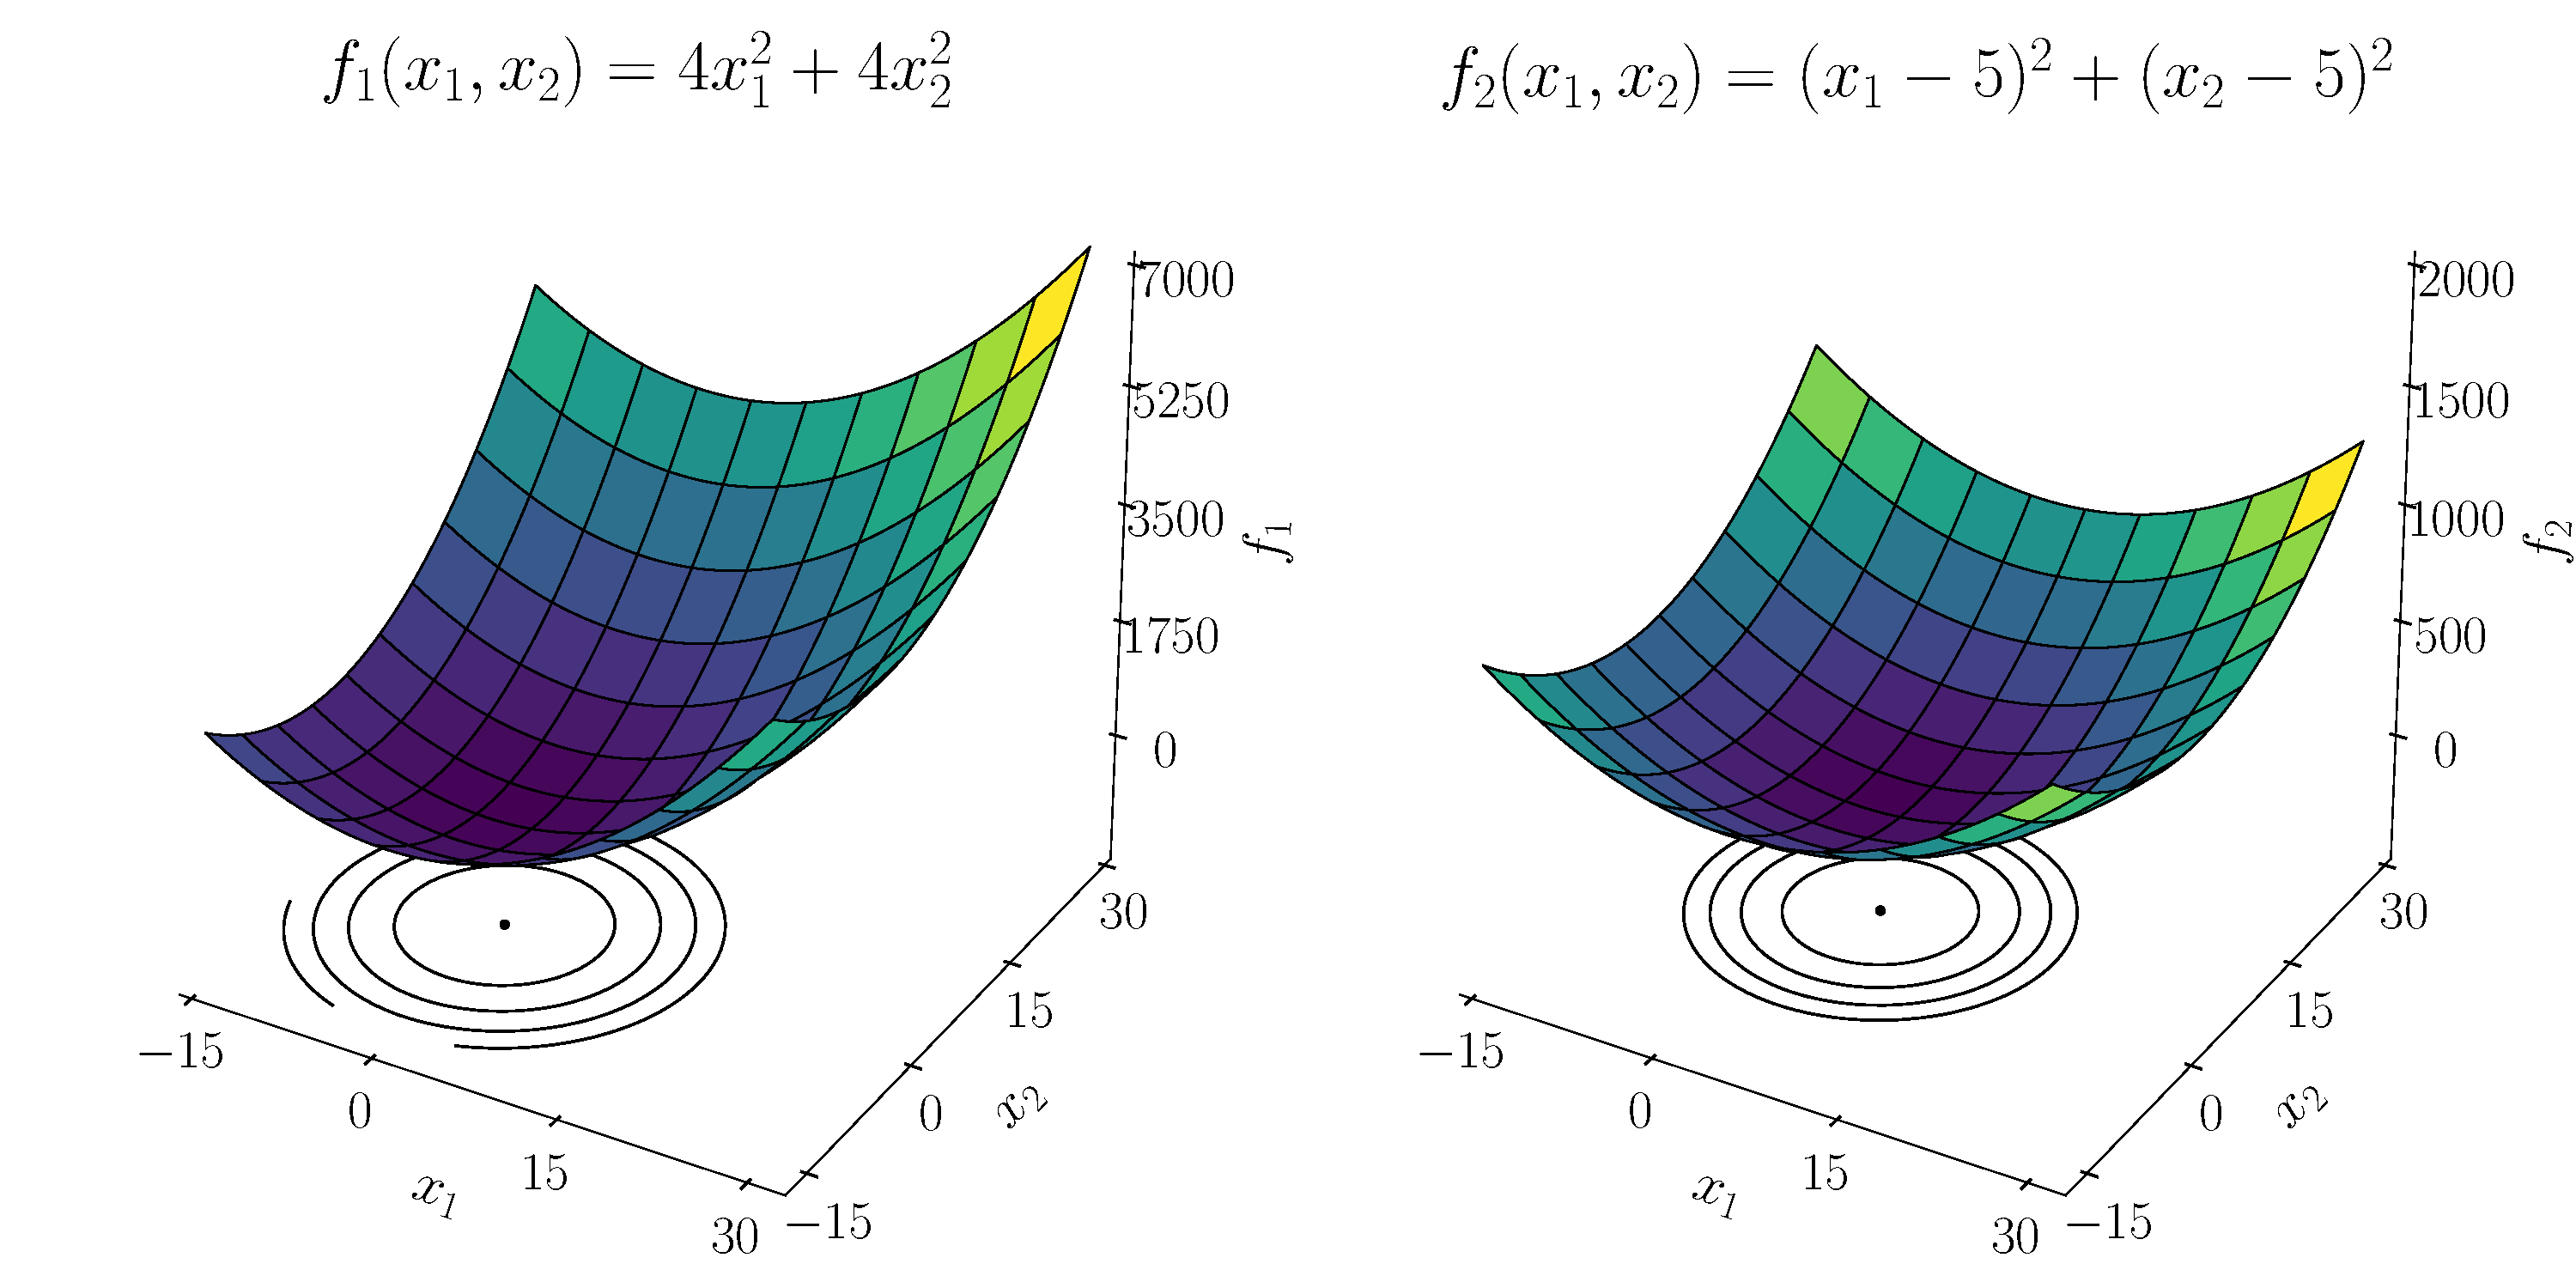
\includegraphics[width=\textwidth]{Figures/2/BK2.pdf}
        \caption{Bihn and Korn test function}
        \label{fig:BihnKorn}
    \end{figure}
    
    As it can be seen in the figure \ref{fig:BihnKorn}, both objective functions are smooth and have defined maximums, but they are not located in the same $\bm{x}$: in the case of $f_1$ the minimum is located in $(0,0)$ and in $f_2$ the minimum is in $(5,5)$. Thus, instead of having one unique solution $\bm{x}$ a set of $\bm{x^*} \in S$ will form the 'optimum' solution. This set of possible values will not be able to optimize both functions at the same time but obtain the better parameters for both cases. From that set of possible solutions, a decision maker should choose the best combination based on previous information. The value of $f(\bm{x^*})$ is the objective vector for the optimum decision vector $\bm{x^*}$.

\subsubsection*{Weighted averaged sum}

    The problem of optimizing multiple objectives at the same time may seem banal: transforming the multi-criteria problem into a weighted sum of the different objective functions is one approach that has been widely used and developed (see \cite{stanimirovic2011linear} and \cite{kim2006adaptive}). This plain aggregating approach consists of:
    
    \begin{equation}
        \begin{array}{cl}
            \textrm{minimize} & F(\bm{x}) = \displaystyle \sum_{m=1}^{k}  w_m f_m(\bm{x}) \\
            \textrm{subject to} & \bm{x} \in S
        \end{array}
        \label{eq:weightedSum}
    \end{equation}
    
    
    This may seem like a good approach. Its main advantage is the simplicity, but the success of the method largely depends on the chosen weights, which value is determined with the relative importance of each objective to the additive objective. It has also problems when dealing with non-convex objective spaces, given that some solutions can't be represented with the average sum \cite{jakob2014pareto} \cite{fonseca1995overview}.

\subsection{Pareto front}

    When there are multiple functions that are to be minimized with a trade-off between them that doesn't allow the existence of a single optimum decision vector $\bm{x}$, Pareto dominance concept arises. Let's assume that there are two feasible solutions that belong to the search space, such that $\bm{x}^1\in S$ and $\bm{x}^2\in S$. 
    
    \newpage
    
    It is said that the solution $\bm{x}^1$ dominates the solution $\bm{x}^2$ when $\bm{x}^1 \prec \bm{x}^2$. The formal definition of the Pareto dominance between two decision vectors is \cite{collette2013multiobjective}:
    
    \begin{equation}
        \bm{x}^1 \prec \bm{x}^2\ \ \ \textrm{if} \ \ \left\{
        \begin{array}{rl}
            f_i(\bm{x}^1) \leq f_i(\bm{x}^2)&  \forall i \in \{1,2,3,...,k\}\\
            f_j(\bm{x}^1) < f_j(\bm{x}^2) & \textrm{for at least one } j \in \{1,2,3,...,k\} 
        \end{array} \right.
        \label{eq:ParetoDominance}
    \end{equation}
    
    The concept of Pareto dominance is shown with a graphical explanation (restricted for 2 objective problems for clarity) in the next figure:
    
    \begin{figure}[h!]
        \centering
        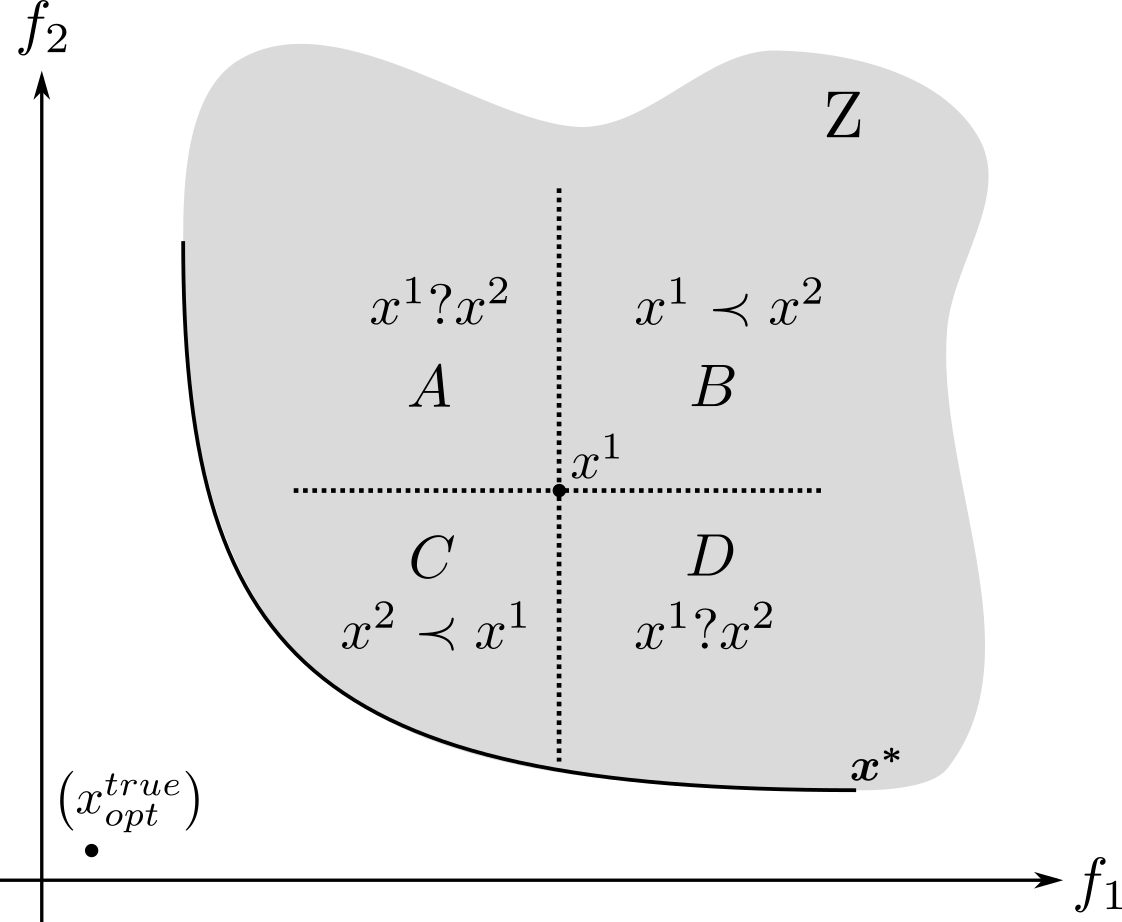
\includegraphics[width=0.75\textwidth]{Figures/2/paretoFront4cuad.png}
        \caption{Pareto front dominance concept example}
        \label{fig:4cuad}
    \end{figure}
    
    Each decision vector $\bm{x}^1$ splits the function space in 4 areas. A decision vector $\bm{x}^2$ (assuming that $\bm{x}^1 \neq \bm{x}^2$) may belong to:
    \begin{itemize}
        \item \textit{Area A} or \textit{Area D}: the relation between $\bm{x}^1$ and $\bm{x}^2$ cannot be determined, given that one performs better in one objective but worse in the other and viceversa.
        \item \textit{Area B}: there is a Pareto dominance relation, having $\bm{x}^1 \prec \bm{x}^2$, where vector $\bm{x}^1$ dominates $\bm{x}^2$.
        \item \textit{Area C}: there is also a Pareto relation between the decision vectors, having $\bm{x}^2 \prec \bm{x}^1$. Thus, $\bm{x}^1$ is dominated by $\bm{x}^2$.
    \end{itemize}
    
    \newpage
    
    If there is one decision vector $\bm{x}^*$ for which there is not any other $\bm{x}$ in \textit{Area C} (i.e. there is not any solution that dominates $\bm{x}^*$) it is said that it is Pareto optimal or non-dominated. The set of Pareto optimal solutions $\bm{x}^*$ is usually called Pareto front or Pareto frontier, which consists of all non-dominated decision vectors (Figure \ref{fig:4cuad}). In can also be seen which is the 'true' optimum value, although given that it is outside the function space $Z$ it is not a valid solution.
    
    The representation of the Pareto front in optimization problems with just two objectives is quite straightforward, as seen in Figure \ref{fig:4cuad}. The Pareto front can be also represented in three dimensions with surfaces, but in high-order multi-objective optimization cases, the representation becomes harder. For those problems, there are other alternatives to the classical representation, e.g. slices of the Pareto front \cite{jaini2017fuzzy} \cite{triantaphyllou2000multi}. Another approach consists of Interactive Decision Maps (IDM) that are techniques that use the concept of the Edgeworth box to show the feasible set expanded by the decision vectors dominated by it \cite{lotov2013interactive}.
    
    Although the optimization process has been described to minimize functions (using $-f_i$ in  case it must be maximized), with the Pareto front all possible combinations of maximization and minimization may be analyzed, as seen in Figure \ref{fig:maxmaxminmin}, where depending the optimization type used, a different zone of the function space is chosen as Pareto front \cite{deb2001multi}:
    \begin{figure}[h!]
        \centering
        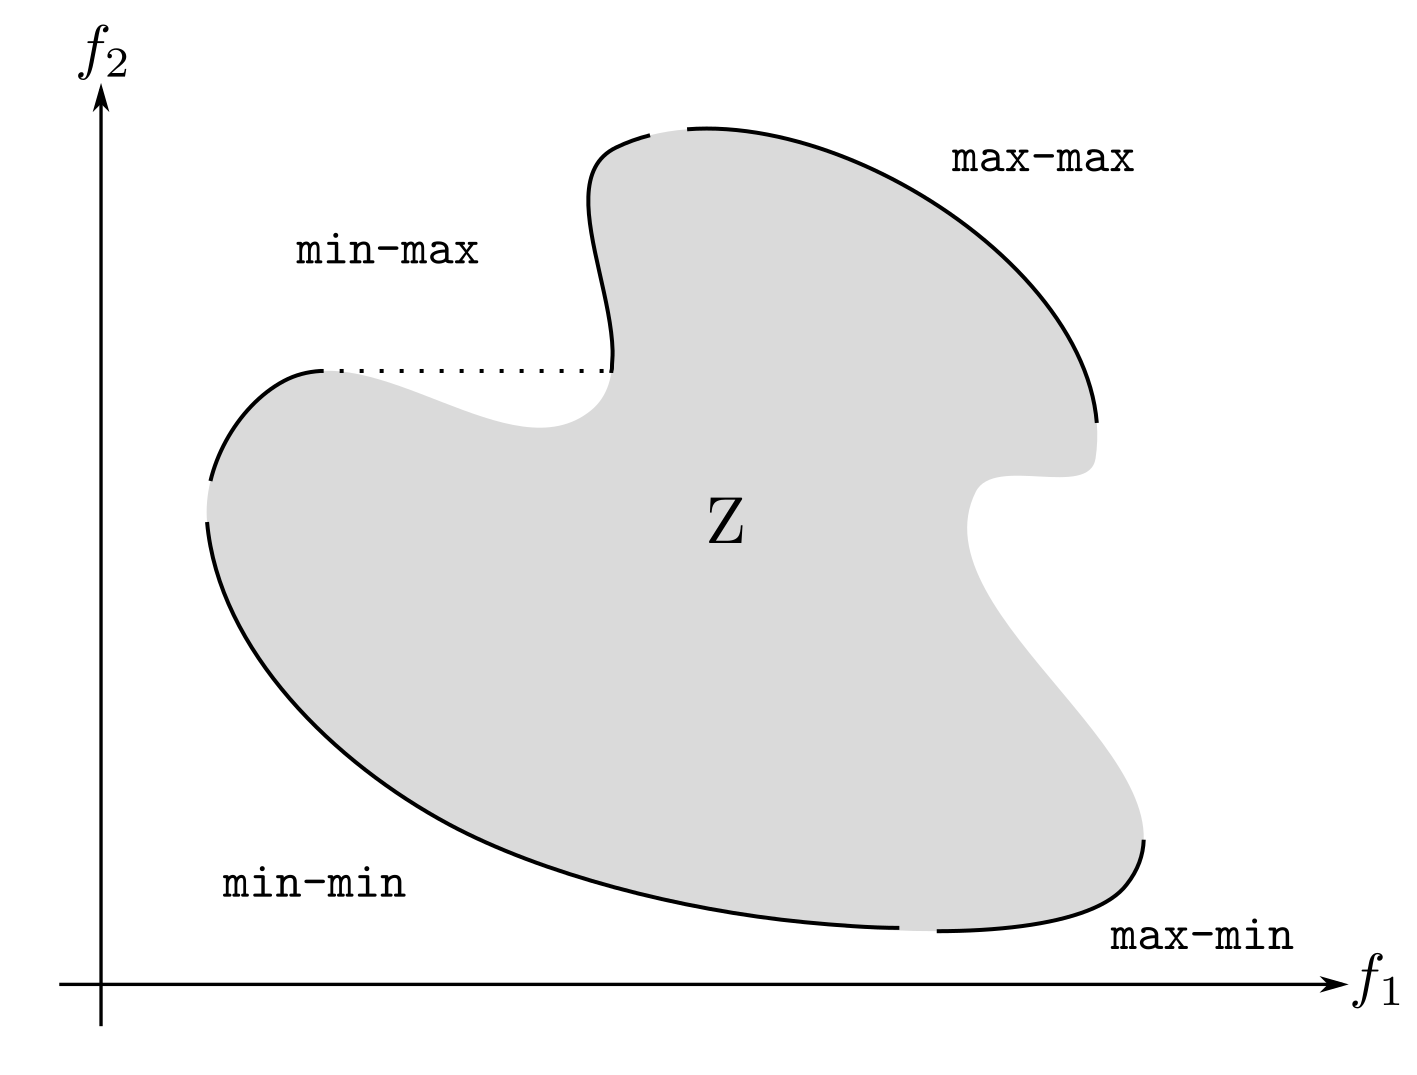
\includegraphics[width=0.75\textwidth]{Figures/2/maxmaxminmin.png}
        \caption{Different Pareto front depending on the type of optimization}
        \label{fig:maxmaxminmin}
    \end{figure}
    
\newpage

\subsection{Approaches for multi-objective optimization}
    One way to solve this kind of multi-objective problems is to create a random set of decision vectors to analyze the best possible the whole search space \cite{li2012momcmc}. The most widely known stochastic techniques are the MCMC (Markov Chain Monte Carlo) methods \cite{spall2005introduction}. They consist of different algorithms such as the Metropolis-Hasting algorithm \cite{altekar2004parallel} or Gibbs sampling \cite{gilks1992adaptive}. MCMC methods provide a fairly good performance with low chance of the worst case performance. As stated by the name, the methods are based on the union of two different techniques \cite{cleverAlgorithms}:
    \begin{itemize}
        \item Monte Carlo methods: they have been traditionally used in statistical physics, they are based on a random sample of the search domain, the deterministic evaluation of the inputs and the aggregation of the results.
        \item Markov chain processes: they provide a probabilistic model for state transitions or moves inside a domain. It is only dependant on the current position to determine the next position, i.e. it has no history retaining. 
    \end{itemize}
    
    Given that error in Monte Carlo methods is reduced $\propto 1/\sqrt{N}$ \cite{caflisch1998monte}, the number of evaluations in order to achieve a good accuracy must be high enough. Thus, the computational resources required to perform an analysis of this kind are considerable.
    
    Other methods of solving this problem consist on physics-inspired algorithms (such as the Chaotic Optimization Algorithm), geography inspired algorithms (as the Imperialistic Competition Algorithm) and social culture inspired algorithms (such as  Memetic Algorithm or the Selfish Gene Algorithm) \cite{cui2017multi}. However, the most popular methods are the biology-inspired algorithms such as evolution based algorithms and swarm-based algorithms, which will be discussed in the following section.

\newpage

\section{Evolutionary computation}

    Talking about artificial intelligence (AI) may seem unrelated to the previous topic at first, but given that evolutionary computation is a sub-field of it, AI must be introduced in order to know how it is structured. Artificial intelligence is a cross-disciplinary field that combines the understanding of the brain from neuroscience, the rise of computers and the new mathematics of information and control theory \cite{cleverAlgorithms}. Therefore, AI is related to the development and investigation of systems that act in an intelligent way. Machine learning is the study of learning processes in different manifestations, i.e. machine learning is another subdivision of artificial intelligence which is focused on problem-solving \cite{michalski2013machine}.
    
    Inside artificial intelligence there are different sub-disciplines, not limited to the ones shown in the next summary: 
    \begin{itemize}
        \item Evolutionary computation: systems based on the Darwinian theory of evolution built on the natural selection of the better genes. There are different kinds of algorithms such as:
            \begin{itemize}
                \item Genetic algorithms: it is a global optimization method with an adaptive strategy. It is based on the understanding of the structure and mechanisms of the genetics.
                \item Genetic programming: it consists of the same principles of genetic algorithms but applied to computer software that adapts and improves its state over time. Instead of coding the lines with the instructions to perform certain tasks, the task is imposed and the evolutionary computation gets the optimum code to perform that task \cite{koza2006genetic} (even improving human coded programs \cite{cramer1985representation}).
                \item Differential evolution: following the same principles as any other evolutionary computation, in this case, a scaled difference mutation is used instead of the typical probability distribution. It is usually used from constrained, large-scale and uncertain optimization problems, as well as multiobjective problems with multiple variables \cite{das2011differential}.
            \end{itemize}
        \item Swarm intelligence: systems based on a large number of not very wise individuals that cooperate and interact with them, obtaining as result a collective intelligence.
        \newpage
        \item Artificial neural networks: systems that are based on a network that behaves as the neurons in the brain: managing the feedback from the environment and achieving some adaptive learning with it.
        \item Fuzzy intelligence: systems that consider a logic with degrees of truth instead of the constrained duality of true and false \cite{klir1996fuzzy}.
    \end{itemize}
    
    
    The classical AI field is divided into two approaches to the problems: \textit{neat AI} and \textit{scruffy AI}. The former uses symbolic representations and logic processes to analyze the given problem, achieving high fidelity in the results. The reductionist analysis is translated into scalability limits: a small increment in the size of the problem leads to an unmanageable increase in the complexity of the system (exaggerated execution time or computing resources). The latter is a descriptive method that takes advantage of the complex, emergent and self-organizing behavior of simple procedures. Using inductive approaches and some stochasticity in the system, the process is more robust when trying to approximate the solution of intractable problems with other methods. Scruffy AI is also known as \textit{metaheuristic}: where \textit{meta-} refers to the higher level strategy of combining different methods or procedures and \textit{-heuristic} is the method that, in order to achieve faster computation time and less resource consuming processes, reduces the precision and quality of the solution (keeping it accurate enough to be sufficient for the case requisites) . These heuristic methods are approximate global solution cannot be ensured), normally non-deterministic and not problem-specific \cite{cleverAlgorithms}.
 
    Conventional algorithms to approach optimization problems (not restricted to multi-objective optimization) are varied: Newton's method, Gradient Descent, Simple method, Nelder-Mead method,... Besides all these well-known techniques, there are algorithms that do not exploit information given from the problem to obtain a solution. This group is usually named as black-box optimization and it includes methods as genetic algorithms (given that only an evaluation of a decision vector is required). These techniques may be applied to a wide range of different problems with small modifications in the algorithm \cite{droste2006upper}. Associated with these black-box algorithms, the \textit{no-free-lunch} theorem states that if one algorithm performs better than other in one particular case, that offset will be reversed for other problems where it will perform worse \cite{wolpert1997no}. This proposition caused pessimism when comparing different optimization techniques, but it can be understood as if each problem is most suitable to certain algorithm that may not be valid for other cases - having to choose the better algorithm for each situation.

\newpage

\subsection{Genetic algorithms overview}
    
    A genetic algorithm (shortened as GA) is a population-based technique that tries to search for solutions to certain problems instead of searching paths for goals. Although searching one solution includes searching the path to achieving that solution, the main target of the algorithm is searching a solution in a large space efficiently instead of developing a decision tree to achieve a goal in all situations \cite{mitchell1998introduction}.
    
    Given that genetic algorithms are based on biological evolution, some biological terminology may be used in the discussion (although mathematical terminology will take precedence). Therefore, before going into the details, these basic terms will be introduced. Cells are the basic element of all living organism and they store the DNA string structured in chromosomes. Each chromosome is divided into genes located in a particular locus of the chromosome, encoding each one gene for a protein. Most parts of the organisms have more than one chromosome per cell. All those possible chromosomes form the genome of the individuals, having that all genes contained inside a genome form the genotype of an organism. 

    There is a close relationship between optimization and genetic algorithms - that is why GA are such a good approach to optimization problems. As it has been mentioned (Figure \ref{fig:twoSpaces}), optimization used two different spaces: parameter space ($\bm{x}$) and the function space ($f(\bm{x})$). In genetic algorithms, there are also two spaces that represent the same concept: \textit{search} space and \textit{fitness} landscape. The search space is the set of all possible states that certain individual or chromosome may have (having each one different genes or components). Fitness landscape is the representation of all possible genotypes with their fitness. The fitness of an individual is a representation of 'how good' its chromosome is, which is translated into the possibilities of having offspring. Genetic algorithms assume that individuals with high fitness will have offspring that will have high fitness too - and it is there where the capabilities of GA relies on.
    
    One aspect that makes genetic algorithms a very broad topic are the two possible ways of encoding the chromosome of each individual: \textit{binary} and \textit{real-valued} (although others as tree encoding or permutation encoding \cite{ronald1995genetic} have been also proposed). Binary encoding is the most common encoding, for both historical reasons and simplicity when dealing with the different operators. However, coding a state with strings of 0 and 1 when dealing with real numbers is unwieldy. In those cases, a real-valued encoding is preferred. This encoding is not limited to the use of float number but also strings of numbers, even combined with letters. The versatility of this encoding makes it widely used and the chosen one for further analysis. 
    
\subsection{Structure of a simple genetic algorithm}
    
    The main operation of a genetic algorithm and its structure will be included in this subsection. A genetic algorithm begins with the initialization of a population. It may be done in a random way, in an equally spaced way or in any other type of sampling of the search space. The \textit{fitness} of the population is evaluated according to the function and objectives selected. Each individual of the population will have a fitness value associated. Then  the three \textit{genetic algorithm operators} are applied:
    
    \begin{itemize}
        \item Selection: this operator selects individuals from the population. There are different types of selection, but the two more common ones are \cite{zhong2005comparison}:
        \begin{itemize}
            \item Roulette wheel selection: random individuals are chosen according to a probability proportional to the fitness value that each individual has.
            \item Tournament method: $n$ uniformly random chosen individuals are faced in a tournament, selecting the one with higher fitness.
        \end{itemize}
        Any selection operator must ensure that the fitter the chromosome, the more times it is selected.
        \item Recombination: two individuals are chosen from the ones selected and are combined, giving rise to (at least) one new individual. As it has already been pointed out, GA assumes that the higher the fitness of the parents, so will be the fitness of the offspring. Recombination tries to increase convergence of the system by joining together points with high fitness. In this recombination phase there are three possibilities that may exist \cite{thevenin2008and}:
        \begin{itemize}
            \item Crossover: some of the genes are taken from one parent and the rest of the genes of the offspring chromosome are taken from the other parent. It is used to increase the diversity.
            \item Average: two parents are chosen and create the chromosome of the offspring with the mean value of each of its genes. This may also be a weighted sum of the parents instead of a plain 50-50 mean.
            \item Survival: it is not exactly recombination but the survival of one of the two chromosomes of the parents. This method takes the chromosome of a parent and saves it in the offspring population. Survival is also known as elitism, given that the elite of the population (sorted by the fitness value) will be preserved along generations.
        \end{itemize}
        \item Mutation: perturbations are applied to each individual in order to ensure variability. The probability of mutation is usually chosen as input, with a value different from zero. The task of mutation is to introduce diversity back into the population. In optimization, this has an especial meaning, given that the GA must move between different optimum locations to analyze the whole domain, so it must be able to leave a local minimum in case it gets stuck in one. Mutation can be applied to a whole chromosome or only to some of its genes. It is a random process, so individuals may not be mutated and keep the chromosomes obtained after recombination.
    \end{itemize}
    
    \begin{figure}[h!]
        \centering
        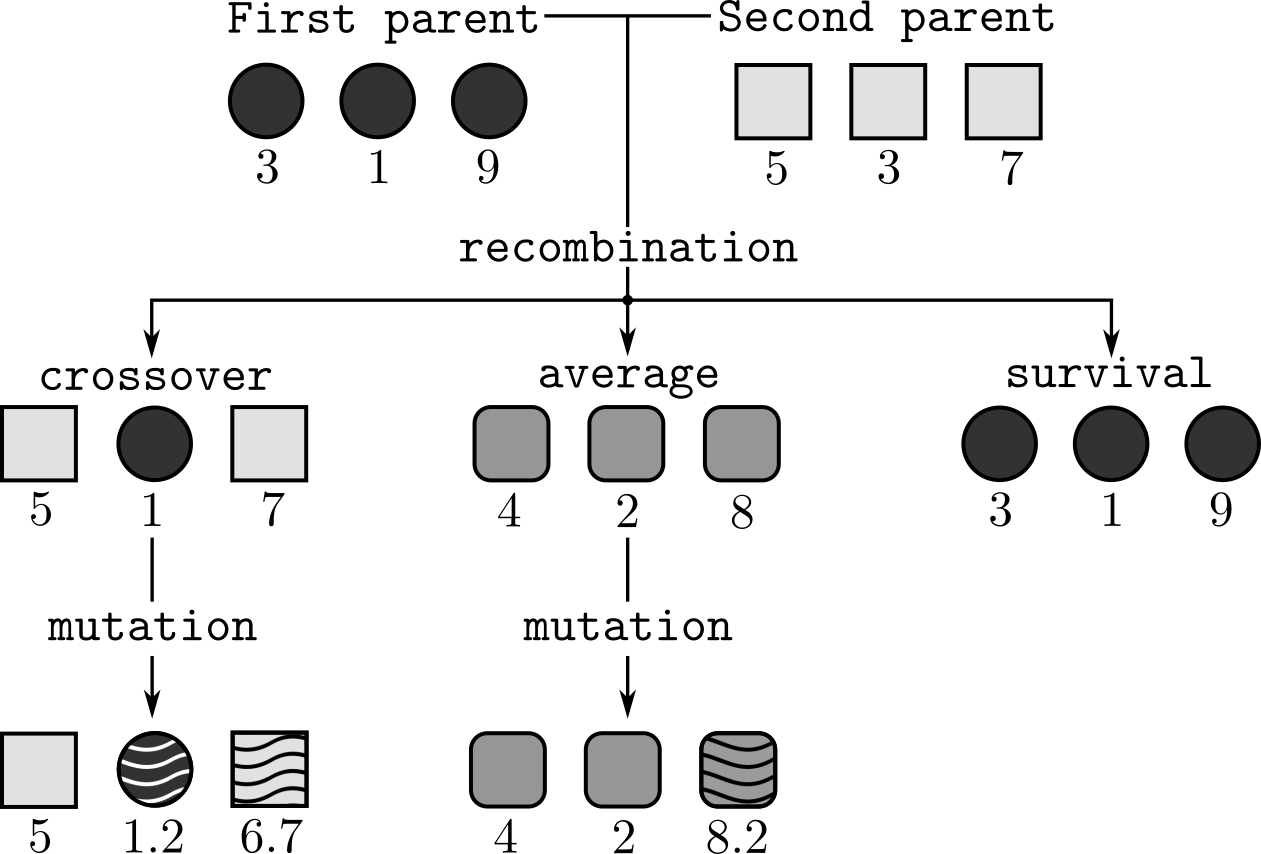
\includegraphics[width=0.8\textwidth]{Figures/2/crossover.png}
        \caption{Recombination and mutation process from two parents}
        \label{fig:crossoverTheory}
    \end{figure}

    Once these three operators have been applied, a new population will arise - having a new generation. That population will undergo the same cycle until one stop condition is matched: it is usually the maximum number of generations or some relative error. For each generation two basic groups must exist: \textit{parents} (individuals that have been chosen to reproduce) and \textit{offspring} (individuals obtained from the combination of the parents). A third group, \textit{elite}, may exist if the genetic algorithm applies the survival operator. Elitism \cite{yager2012introduction} has been proved to have a considerable impact on performance, because it avoids wasting time in discovering again zones that have been already discarded as not valid. The same individual may be part of several groups at the same time, i.e. there are algorithms that compare the value of parents and offspring to keep the better for recombination and mutation.

    \newpage
    
    Genetic algorithms may be mathematically formalized for simple genetic algorithms (see \cite{goldberg2006genetic} \cite{vose1991punctuated} \cite{whitley1993executable}), being able to analyze the dynamics of the system. GA are used for optimization problems, where once the optimum value is found, the state does not move from there. This kind of points are fixed points and in genetic algorithms are achieved once a population has completely converged to individuals with the same fitness. If a population does not have all individuals at the maximum fitness level, a small perturbation may move the solution from the fixed point. This situation causes \textit{punctuated equilibia} in fitness evolution: long periods of no improvement with quick rises in the fitness. Although these effects have to be rigorously quantified under different models, the implications are that a large enough number of generations must be computed to achieve a high fitness. The main assumption is that the population has an infinite size, which may lead to unexpected behaviors due to sampling errors in a genetic algorithm with a limited population size. 
    
    The basic procedure of a genetic algorithm is listed below:
    \begin{algorithm}
        \caption{Simple Genetic Algorithm}\label{alg:simpleGApseudoCode}
        \begin{algorithmic}[1]
        \State initialize \textit{population}
        \While {stopCriterion \textbf{not} reached }
            \State calculate \textit{fitness} of \textit{population}
            \State select \textit{bestIndividuals} from \textit{population}
            \State \textit{newPopulation} $\leftarrow$ mutation $\leftarrow$ crossover \textit{bestIndividuals}
            \State \textit{population} $\leftarrow$ \textit{newPopulation}
        \EndWhile
        \end{algorithmic}
    \end{algorithm}

\subsection{Why do genetic algorithms work?}

    Although a genetic algorithm is procedure simple to describe and code, its behavior may be complicated and there are still many questions about how do they really work. A genetic algorithm results in complex and robust search method by implicitly sampling hyperplane partitions of a search space \cite{whitley1994genetic}.
    The genetic algorithm works by discovering and recombining good \textit{building blocks} of solutions, given that a good building block will make up a good building block.
    Holland's book \cite{john1992holland} refers to this building blocks as \textit{schemas} that defines hyperplanes ('planes' of various dimensions). One schema on its own does not provide enough information, that is where the population-based search concept is critical, given that many hyperplanes are evaluated at the same time. The cumulative effects of evaluating a population of points will provide enough information about any particular subset of hyperplanes.

\newpage

\subsection{Genetic algorithms for multi-objective optimization}
        
    Due to the similarities between genetic algorithms and multiobjective optimization, there are a lot of existing and well-tested methods that combine both. The ability of a GA to search in different regions of the solution space in a highly parallel fashion makes it a good tool for problems with non-convex, discontinuous and multi-modal solution spaces. Undoubtedly, genetic algorithms are one of the most popular heuristic approaches to multi-objective optimization. 
    In the next table, the most popular genetic algorithms and some of its special features are listed \cite{konak2006multi}:
    \begin{table}[h!]
    \centering
    \caption{Different genetic algorithms for multi-objective optimization}
    \begin{tabular}{lllcc} 
    \hline
    \textbf{Algorithm} & \textbf{Fitness assignment} & \textbf{\begin{tabular}[c]{@{}l@{}}Diversity~\\mechanism\end{tabular}} & \textbf{Elitism} & \textbf{\begin{tabular}[c]{@{}l@{}}External~\\population\end{tabular}} \\ 
    \hline
    VEGA & \begin{tabular}[c]{@{}l@{}}Each population is~\\evaluated with respect~\\to a different objective\end{tabular} & No & No & No \\ 
    \hline
    MOGA & Pareto ranking & \begin{tabular}[c]{@{}l@{}}Fitness sharing ~\\ by niching\end{tabular} & No & No \\ 
    \hline
    PESA & No fitness assignment & Cell-based density & Yes & Yes \\ 
    \hline
    NSGA & \begin{tabular}[c]{@{}l@{}}Ranking based on~\\non-domination sorting\end{tabular} & Niching & No & No \\ 
    \hline
    NSGA-II & \begin{tabular}[c]{@{}l@{}}Ranking based on~\\non-domination sorting\end{tabular} & Crowding distance & Yes & No \\ 
    \hline
    SPEA &  \begin{tabular}[c]{@{}l@{}}Ranking based ~\\ on external archive ~\\ of non-dominated \end{tabular} & \begin{tabular}[c]{@{}l@{}}Clustering to ~\\ truncate external ~\\ population\end{tabular} & Yes & Yes \\ 
    \hline 
    SPEA-2 & Strength of dominators & \begin{tabular}[c]{@{}l@{}}Density based of~\\ $k$ nearest\end{tabular} & Yes & Yes \\ 
    \hline 
    DMOEA & Cell-based ranking & \begin{tabular}[c]{@{}l@{}}Cell-based~\\density\end{tabular} & Yes & No \\
    \hline
    \end{tabular}
    \label{table:differentMOGA}
    \end{table}
    Many other genetic algorithms exist and have been also tested, but only the most important and used have been listed above. There are some nomenclature that has not been introduced and it must be explained before analyzing the advantages and disadvantages of each method:
    \begin{itemize}[label={--}]
        \item \textbf{Fitness assignment}: procedure followed to assign the fitness to the individuals of each generation. It may be based on a wide range of methods of assigning.
        \item \textbf{Diversity mechanism}: techniques used to promote the diversity of the solutions, i.e. the spread of individuals to cover the whole search and function space.
        
        \newpage
        
        \item \textbf{Elitism}: for a single-objective genetic algorithm, elitism consists on saving the best solution for the next generation. However, in multi-objective optimization, all non-dominated solutions that form the Pareto front are considered elite solutions but elitism is not as straightforward as in single objective. Although earlier genetic algorithms did not include elitism, most recent strategies include it because it outperforms non-elitist counterparts.
        \item \textbf{External population}: proposes to save in a list the elitist individuals for each generation. Apart from being a computationally expensive task, the size of the list may grow too much. In order to avoid that, pruning techniques have been proposed to limit the maximum size of the elitist population.
        \item \textbf{Fitness sharing}: a method used to encourage the search in unexplored zones of a Pareto front by artificially reducing the fitness of the solutions in densely populated areas with some penalization method.
        \item \textbf{Niching}: technique consisting on segmenting the population in disjoint sets so each member may go to different zones, in order to cover more than one local optima. It is a highly used technique to widen the whole search space in fewer generations due to the splitting of the population.
        \item \textbf{Cell-based density}: consists on dividing the objective space into $K$ cells, computing the density of each cell and assigning that value to each solution in the cell. Then, the most populated cells are penalized in a similar way as fitness sharing.
        \item \textbf{Crowding distance}: technique that eliminates the necessity of a user-defined parameter such as $\sigma_{shared}$ or the $k$ nearest neighbors. It computes the distance between the points of the Pareto front and uses that distance for the selection process.
        \item \textbf{Strength of dominators}: assignment of the fitness value according to the number of individuals that dominate each individual.
    \end{itemize}
    
    Once the terminology used in this kind of genetic algorithms is known, a brief discussion about each one of them will be held. Main advantages and disadvantages will be presented and shown in order to decide which will be the most optimum algorithm:

    \newpage

    \begin{itemize}
        \item VEGA (Vector Evaluated Genetic Algorithm): it was the first genetic algorithm designed for multi-objective optimization. Although the easy implementation, its main disadvantage is that it tends to converge to the extreme of each objective, losing an important part of the Pareto front.
        \item MOGA (Multi-Objective Genetic Algorithm): it is a simple extension of a genetic algorithm for single objective. However, it has problems related to the niche size parameter and the slow convergence.
        \item PESA (Pareto Envelope-based Selection Algorithm): it is easier to implement and (if done correctly) it is computationally efficient. The main problem is that the performance and the success of the method depend on the cell sizes and some previous knowledge about the objective space is required.
        \item NSGA (Non-dominated Sorting Genetic Algorithm): it has an extremely fast convergence but also major problems related to the niche size parameter.
        \item NSGA-II (Non-dominated Sorting Genetic Algorithm II): efficient, well tested and single parameter ($N$) method. The main disadvantage is that the crowding distance works only in the objective space.
        \item SPEA (Strength Pareto Evolutionary Algorithm): well test method without any parameter for clustering. Its inconvenient is that the clustering algorithm is quite complex.
        \item SPEA-2 (Strength Pareto Evolutionary Algorithm 2): it is an improved version of the SPEA that also makes sure that the extreme points of the Pareto front are preserved (in order to increase both the diversity and the convergence). The drawback of the method is that the fitness and density calculation are highly computationally expensive.
        \item DMOEA (Decomposition-based Multi-Objective Evolutionary Algorithm): it is a method that combines some efficient techniques to update cell densities and adaptative approaches to set the genetic algorithm parameters. The main downside is its complicated implementation.
    \end{itemize}
    
From this list of some of the most well-known genetic algorithms for multiobjective optimization, one will be chosen for the implementation and application to the CFD cases. There are some characteristics that must exist in the genetic algorithm in order to be used successfully in the cases.

\newpage

The desired characteristics that a GA  must have for being applied successfully to CFD cases are:
\begin{itemize}
    \item Elitism: keeping the best individuals along generations has shown that the convergence of the solution is faster and requires less number of generations. Thus, it is very important that the algorithm chosen has elitism, given that each individual may have an evaluation time of minutes due to the CFD simulation. 
    \item Avoid user-defined parameters: achieving the correct solution is usually directly related to the value that those parameters have, so it is interesting to choose a genetic algorithm that does not have user-defined parameters. Some of these parameters include the $k$ nearest individuals or the size of the cells when performing the fitness evaluation. 
    \item Well-tested method: an algorithm whose performance has been tested and is above certain limit when talking about convergence to a solution is preferable with respect to a newer method that has not been tested yet. 
    \item Efficient and low resources consuming: given that the computational fluid dynamics simulations will be running for long periods of time, increasing the computational resources required for evaluating the fitness and performing the different operators is not a great way of approaching the problem.
    \item Straightforward implementation: given that the code will be implemented in Python, it is also interesting to have an algorithm whose coding may be done in a simple way and with a high level of parallelization.
\end{itemize}
Analyzing the algorithms in the table \ref{table:differentMOGA}, the one that meets all the requirements is the NSGA-II. 

\subsection{Non-dominated Sorting Genetic Algorithm II)}
The algorithm that was chosen to be implemented and used in the different computer fluid setups is the NSGA-II. This algorithm is described in \cite{deb2002fast} where the algorithm is presented as a review of the first version of the NSGA. Some characteristics that make this algorithm suitable for this study have been already mentioned. However, the potential of the algorithms lays in fitness evaluation and the way it handles the populations of parents and offspring. A combination of all these parameters is what makes this algorithm so attractive for this study. 

\newpage
The main features of the NSGA-II are:
\begin{itemize}
    \item Fast non-dominated sorting: the points of an evaluation are sorted depending on the Pareto front in which they are located on. The points in the non-dominated Pareto front will have the greater fitness possible, while the points with higher values in the functions $f_1$ and $f_2$ have a smaller fitness. Selection is performed based on the number of the Pareto front in which the individual is located: the higher the fitness, the less dominated the individual will be by other individuals and the greater possibilities will it have to be selected.
    \begin{figure}[h!]
        \centering
        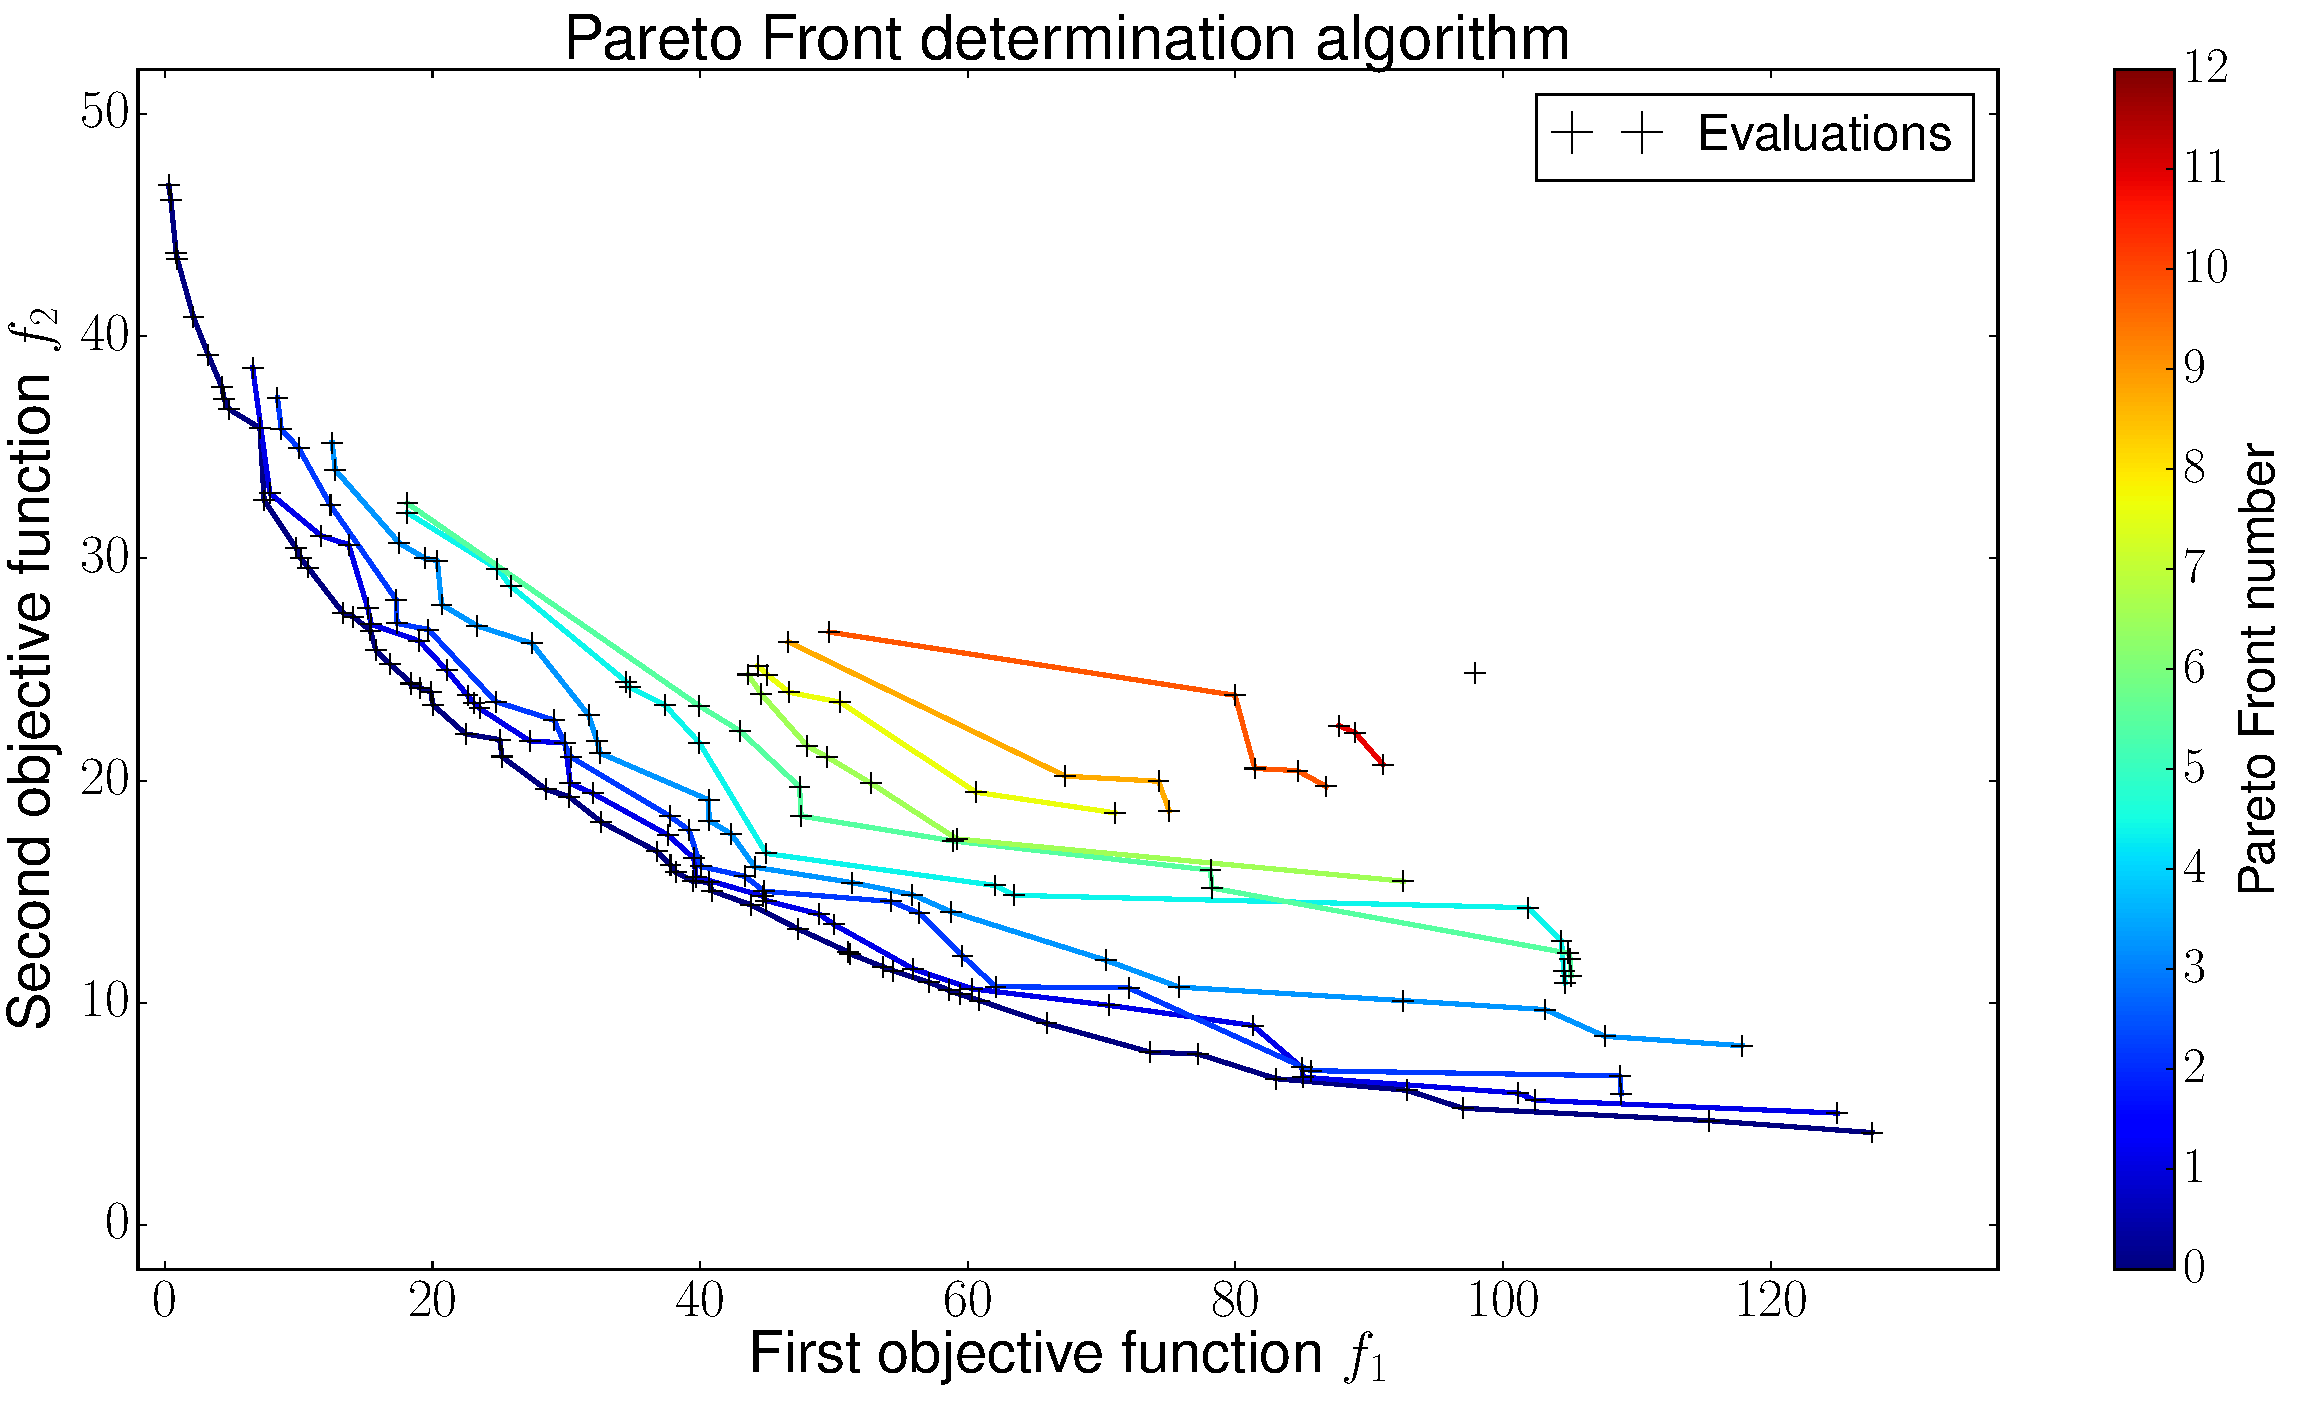
\includegraphics[width=0.85\textwidth]{Figures/2/fastNonDominatedSort.pdf}
        \caption{Fast non-dominated sorting}
        \label{fig:fast-nondominated-sorting}
    \end{figure}
    \item Crowding distance: if a selection is performed with a binary tournament ($k=2$) there are chances for two individuals of the same Pareto front to be in the tournament facing each other. Given that for the points in the same Pareto front, the value of the fitness is the same, there must exist another parameter or value used to break the tie. Crowding distance is used for that purpose, breaking possible ties in the selection process. It is assigned based on the distance to the closest point in the same Pareto front, having a higher crowding distance if the point is located in a low-density area. If the point is located in a dense area, the crowding distance will be smaller having, therefore, smaller chances of being chosen. The extrema points of the Pareto front have a crowding distance of $\infty$, so they are always chosen. In the Figure \ref{fig:crowding_distance} it can be seen how points in less dense areas have a greater crowding distance.
    \begin{figure}[h!]
        \centering
        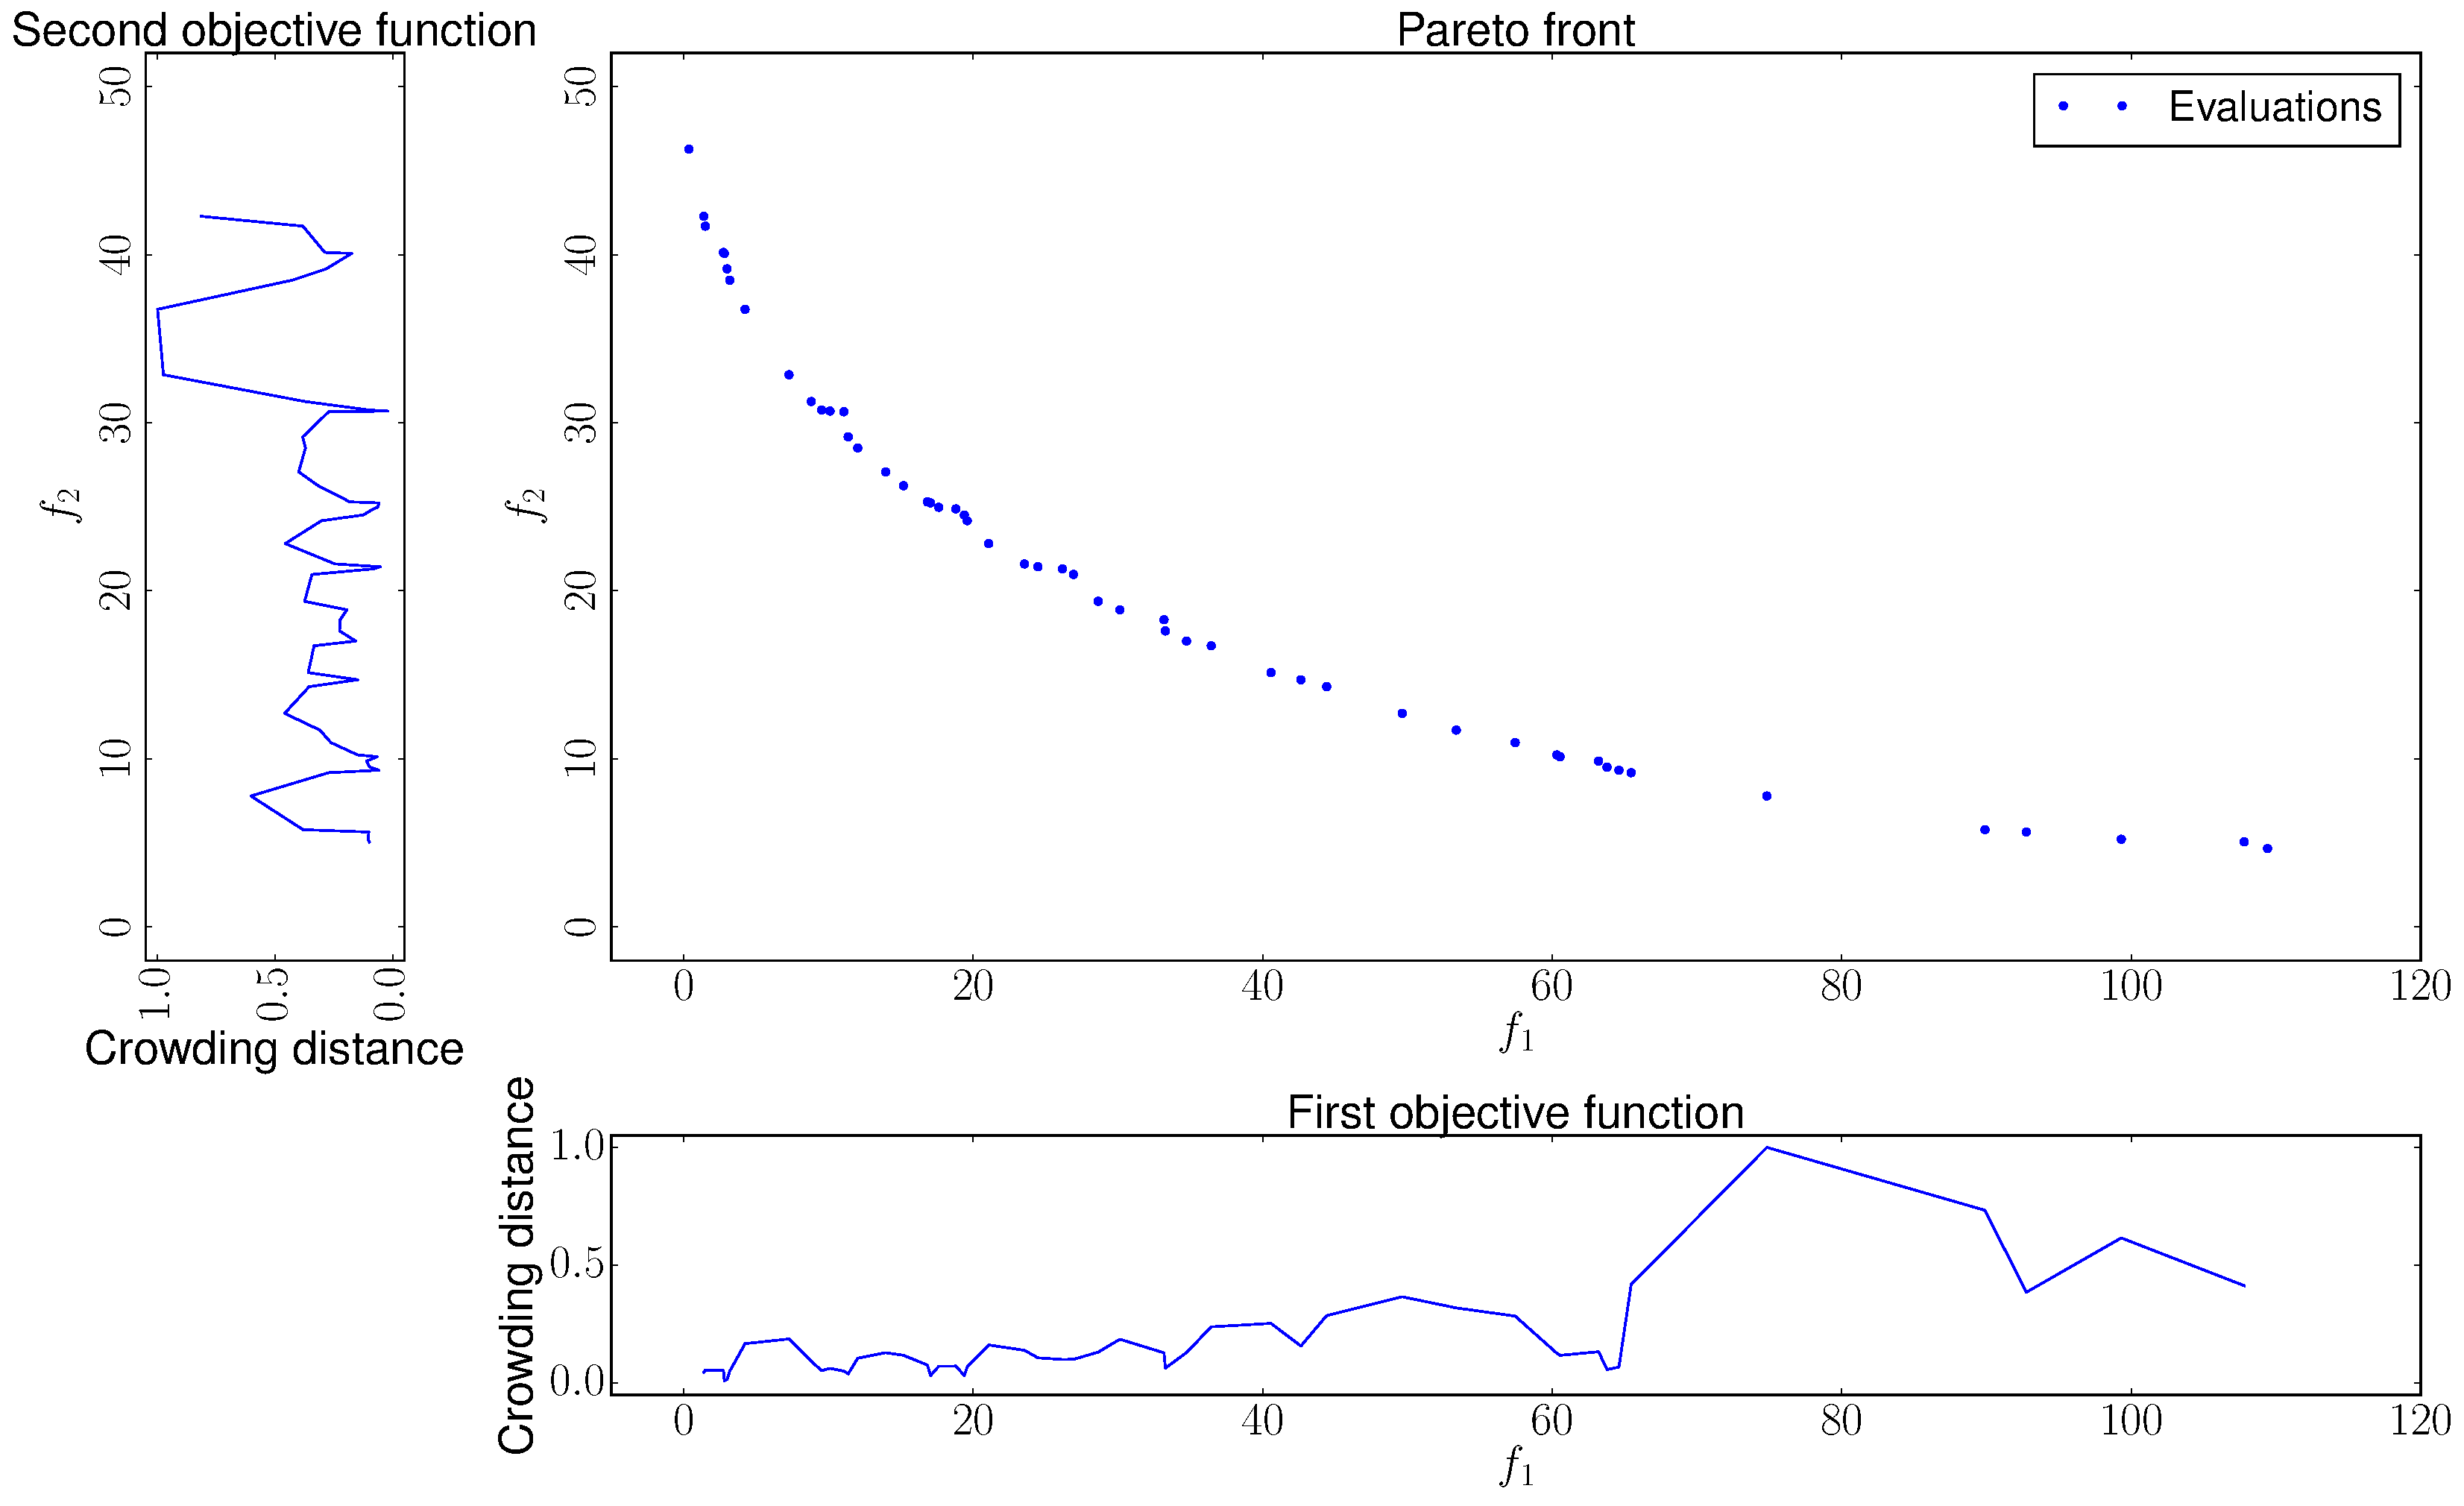
\includegraphics[width=0.95\textwidth]{Figures/2/crowdingDistance.pdf}
        \caption{Crowding distance assignment}
        \label{fig:crowding_distance}
    \end{figure}
    \newpage
    \item Preselection process: these two ways of sorting a population allow a preselection process (prior to the classical selection, recombination and mutation processes) to increase the convergence of the method. It begins with a parent population $P_t$ of size $N$ which yields an offspring population $Q_t$ of size $N$. These two populations are combined in the same set (having a size of $2N$), which is sorted according to the non-dominated sorting explained above (Figure \ref{fig:fast-nondominated-sorting}). The whole set of both parents and offspring are sorted depending on the Pareto front they are located in. Provided that the size of the new population should be $N$, the less dominated Pareto fronts that fit completely the new population will go directly without going through any other process. Once the following Pareto front will not fit completely the new population $P_{t+1}$, the set is sorted with the crowding distance. Thus, from the last Pareto front, only the points with higher crowding distance will be selected for the parent population $P_t+1$. The most rear fronts will not be selected for the new population as well as the lower crowding distance individuals from the last Pareto front. Those points are just rejected. Population $P_{t+1}$ will undergo selection, recombination and mutation to yield population $Q_{t+1}$, closing this way the loop. This is an indirect way of performing elitism given that the best individuals are taken from the previous generation ($P_t$).
        \begin{figure}[h!]
        \centering
        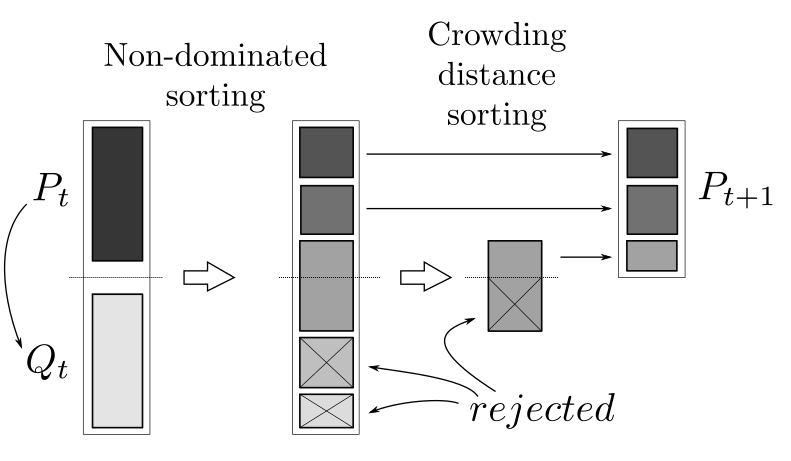
\includegraphics[width=0.9\textwidth]{Figures/2/preselection5.png}
        \caption{Preselection process for a parent population $P_t$}
        \label{fig:preselection process}
    \end{figure}
\end{itemize}
    
The main loop of the genetic algorithm combines all procedures shown before, having the next diagram:

\begin{figure}[h!]
        \centering
        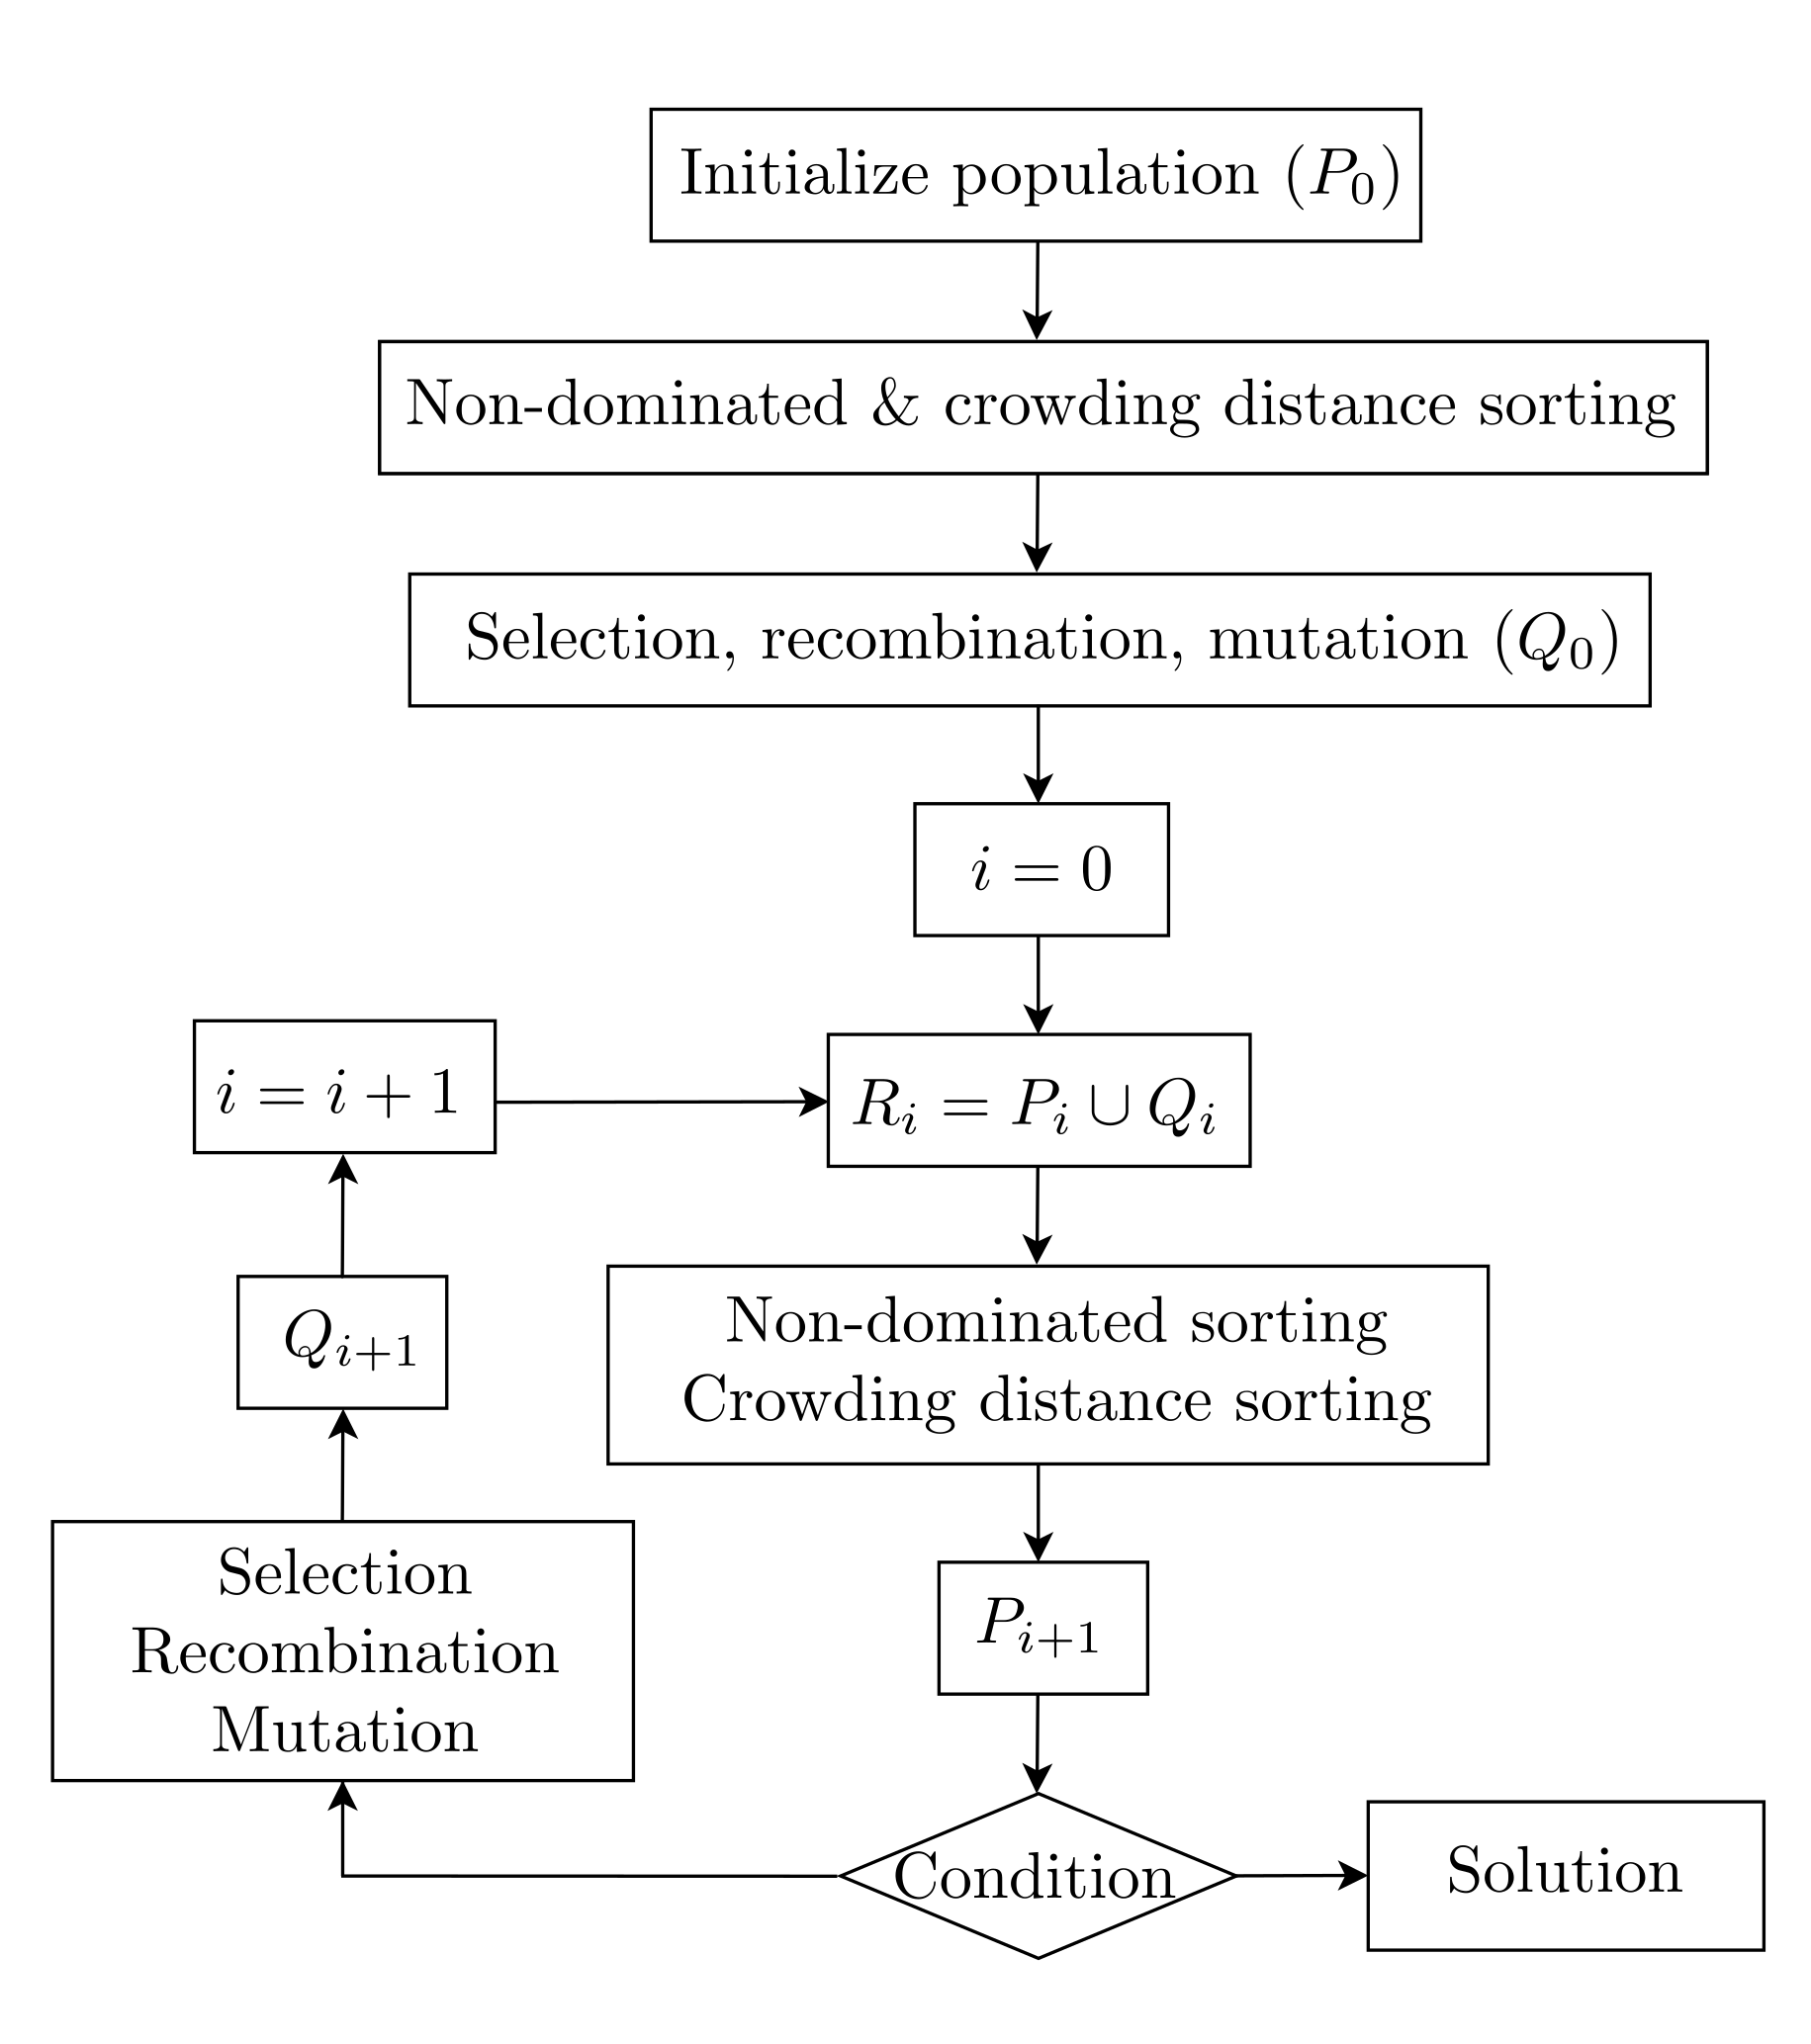
\includegraphics[width=0.6\textwidth]{Figures/2/NSGAflow.png}
        \caption{Chart flow of the NSGA-II algorithm }
        \label{fig:chartFlowNSGAII}
\end{figure}

\newpage

\section{Computer Fluid Dynamics}

Computer fluid dynamics is the analysis of systems involving especially fluid flow (but also heat transfer and chemical reactions) with computer-based simulations. The techniques are very powerful and they may be applied to a wide range of industrial applications. Although other computer-based simulation, such as stress analysis codes, have a greater capability than CFD codes (due to the incredible complexity of the underlying behavior of fluid flows), the use of CFD is essential in every aspect of the design of a new concept or product. The investment in a CFD code is smaller than the minimum cost of the required hardware for an experimental setup (having even some CFD codes that are completely free). 

Almost all CFD codes work in the same fashion, having very differentiated steps \cite{versteeg1995computational}:
\begin{itemize}
    \item Pre-processor: in the step, the setup of the problem is defined: the computational domain is created with a grid or mesh formed by different cells or control volumes. The set of equations to be solved and the fluid properties are selected in this step. Also, the conditions at the boundary of the domain are established. 
    \item Solver: there are different numerical techniques available for approaching these problems: finite difference (especially the finite volume method), finite element and spectral methods. The numerical algorithm consists on a series of steps: the integration of the governing equation of fluid flow, discretization of the resulting integral equation into an algebraic system of equations and the solution of that algebraic system of equations. 
    \item Post-processor: the output obtained in the solver phase is analyzed and data is extracted in order to draw some conclusions. With the increase of graphic capabilities of engineering workstations, a lot of versatile data visualization tools are used to present data in a more visual way. 
\end{itemize}

The set of governing equations of the flow of a compressible Newtonian fluid that is solved in a computer fluid dynamics code is formed by five partial differential equations (PDEs) with two algebraic equations that supplement the five PDEs. The equations are listed in
\ref{table:cfdEqs}.

\newpage

\begin{table}[htb]
\centering

\caption{Equations of a compressible Newtonian fluid} \label{table:cfdEqs}

\begin{tabular}{
    >{\linespread{1.}\selectfont}m{3.cm}
    @{}
    m{12cm}
    @{}
}

Continuity &
  \tableequation{
    \dfrac{\partial \rho}{\partial t} + \text{div} (\rho \bm{u}) = 0
  \label{eq:continuity}} \\

x-momentum &
  \tableequation{
    \dfrac{\partial (\rho u)}{\partial t} + \text{div} (\rho u \bm{u}) = -\dfrac{\partial p}{\partial x}+\text{div}(\mu \ \text{grad}\ u) +S_{M_x} 
  \label{eq:xmomentum}} \\

y-momentum &
  \tableequation{
    \dfrac{\partial (\rho v)}{\partial t} + \text{div} (\rho v \bm{u}) = -\dfrac{\partial p}{\partial y}+\text{div}(\mu \ \text{grad}\ v) +S_{M_y} 
  \label{eq:ymomentum}} \\

z-momentum &
  \tableequation{
    \dfrac{\partial (\rho w)}{\partial t} + \text{div} (\rho w \bm{u}) = -\dfrac{\partial p}{\partial z}+\text{div}(\mu \ \text{grad}\ w) +S_{M_z} 
  \label{eq:zmomentum}} \\

Energy &
  \tableequation{
    \dfrac{\partial (\rho i)}{\partial t} + \text{div} (\rho i \bm{u}) = -p\ \text{div}\ \bm{u} +\text{div}(k \ \text{grad}\ T) + \bm{\Phi} +S_i
  \label{eq:energy}} \\

\begin{tabular}{@{}c@{}}Equations \\ of state\end{tabular} &
\tableequation{p=p(\rho,T) \text{ and } i=i(\rho, T)\label{eq:stateEqs}}  \\

 & \tableequation{(\text{for a perfect gas } p=\rho RT \text{ and } i=C_v T )}\\

\end{tabular}

\end{table}

In these equations $\rho$ represents the density of the flow, $\bm{u}$ is the velocity vector with its three components $\bm{u}=(u,v,w)$, $t$ is time, $p$ is the pressure, $\mu$ is the dynamic viscosity, $(x,y,z)$ represent spatial components, $i$ is the internal energy, $k$ is the heat conduction coefficient and $T$ is the temperature. Equations \ref{eq:xmomentum}, \ref{eq:ymomentum} and \ref{eq:zmomentum} have a momentum source $S_M$, while \ref{eq:energy} has an internal energy source term $S_i$ and a dissipation function $\bm{\Phi}$. 

To solve this system of equations, initial conditions and boundary conditions must be established for the case. Depending on the setup to be solved, this system may be simplified down to a more simpler system with fewer variables and equations (for example, by reducing the 3D analysis in a 2D case or doing a steady state solution where the temporal terms are neglected).